\documentclass[hyperref={pdfpagelabels=false}]{beamer}
\usepackage{lmodern}
\usetheme{Berlin}
\definecolor{UniRed}{RGB}{255,0,0}
\definecolor{UniWhite}{RGB}{255,255,255}
\setbeamercolor{eecks} {bg=UniRed, fg=UniWhite}
\title{\textsc{RoboSoccer} Project Plan}  
%\author{Sascha Frank} 
\author{
  Hofbauer, Markus\\
  \and
  Jiang, He \\
  \and
  Meyer, Kevin\\
  \and
  Schmidt, Benedikt\\
  \and
  Wirnshofer, Florian
}
\date{\today} 
\begin{document}
\begin{frame}
\titlepage
\end{frame} 

%
\begin{frame}
\frametitle{Table of contents}
\tableofcontents
\end{frame} 

\section{Definition of Project Objectives} 
\begin{frame}
	\frametitle{Definition of Project Objectives} 
	
	\begin{beamercolorbox}[shadow=true, rounded=true]{eecks}
		\centering		
		\Large{Win the \textsc{RoboSoccer} Championship}
	\end{beamercolorbox}
	\vspace{1cm}
	\begin{block}{Required Objectives}
		\begin{itemize}
			\item Implementation of low and mid-level robot controls.
			\item Implementation of an advanced artificial intelligence.
			\item Obey the \textsc{RoboSoccer} rules.
			\item Implementation of a penalty shoot-out mode.
		\end{itemize}
	\end{block}
\end{frame}

\section{Framework and Procedure} 


\begin{frame}
	\frametitle{Team Members}
	\begin{itemize}
		\item  Hofbauer Markus
  		\item Jiang He 
 		\item Meyer Kevin
  		\item Schmidt Benedikt
  		\item Wirnshofer Florian
	\end{itemize}
\end{frame}

\begin{frame}
	\frametitle{Team Organisation}
	Internal Communication\\
	\begin{itemize}
		\item  Team Discussion Board \\
		(phpBB: \textit{https://forum.kevin-meyer.de})
  		\item Email
	\end{itemize}
	\vspace{0.75cm}	
	Meeting on a weekly basis.\\
	\vspace{0.75cm}
	Additional meetings on demand.
\end{frame}

\begin{frame}
	\frametitle{Hardware} 
	\begin{itemize}
		\item Three \textsc{Pololu 3Pi} robots per team.
		\item Image acquisition using a camera above the playground.		
		\item Localization based on computer vision algorithms.
		\item Communication via dedicated real-time server and a \textsc{Bluetooth} interface.
	\end{itemize}
	\begin{figure}
		\centering
		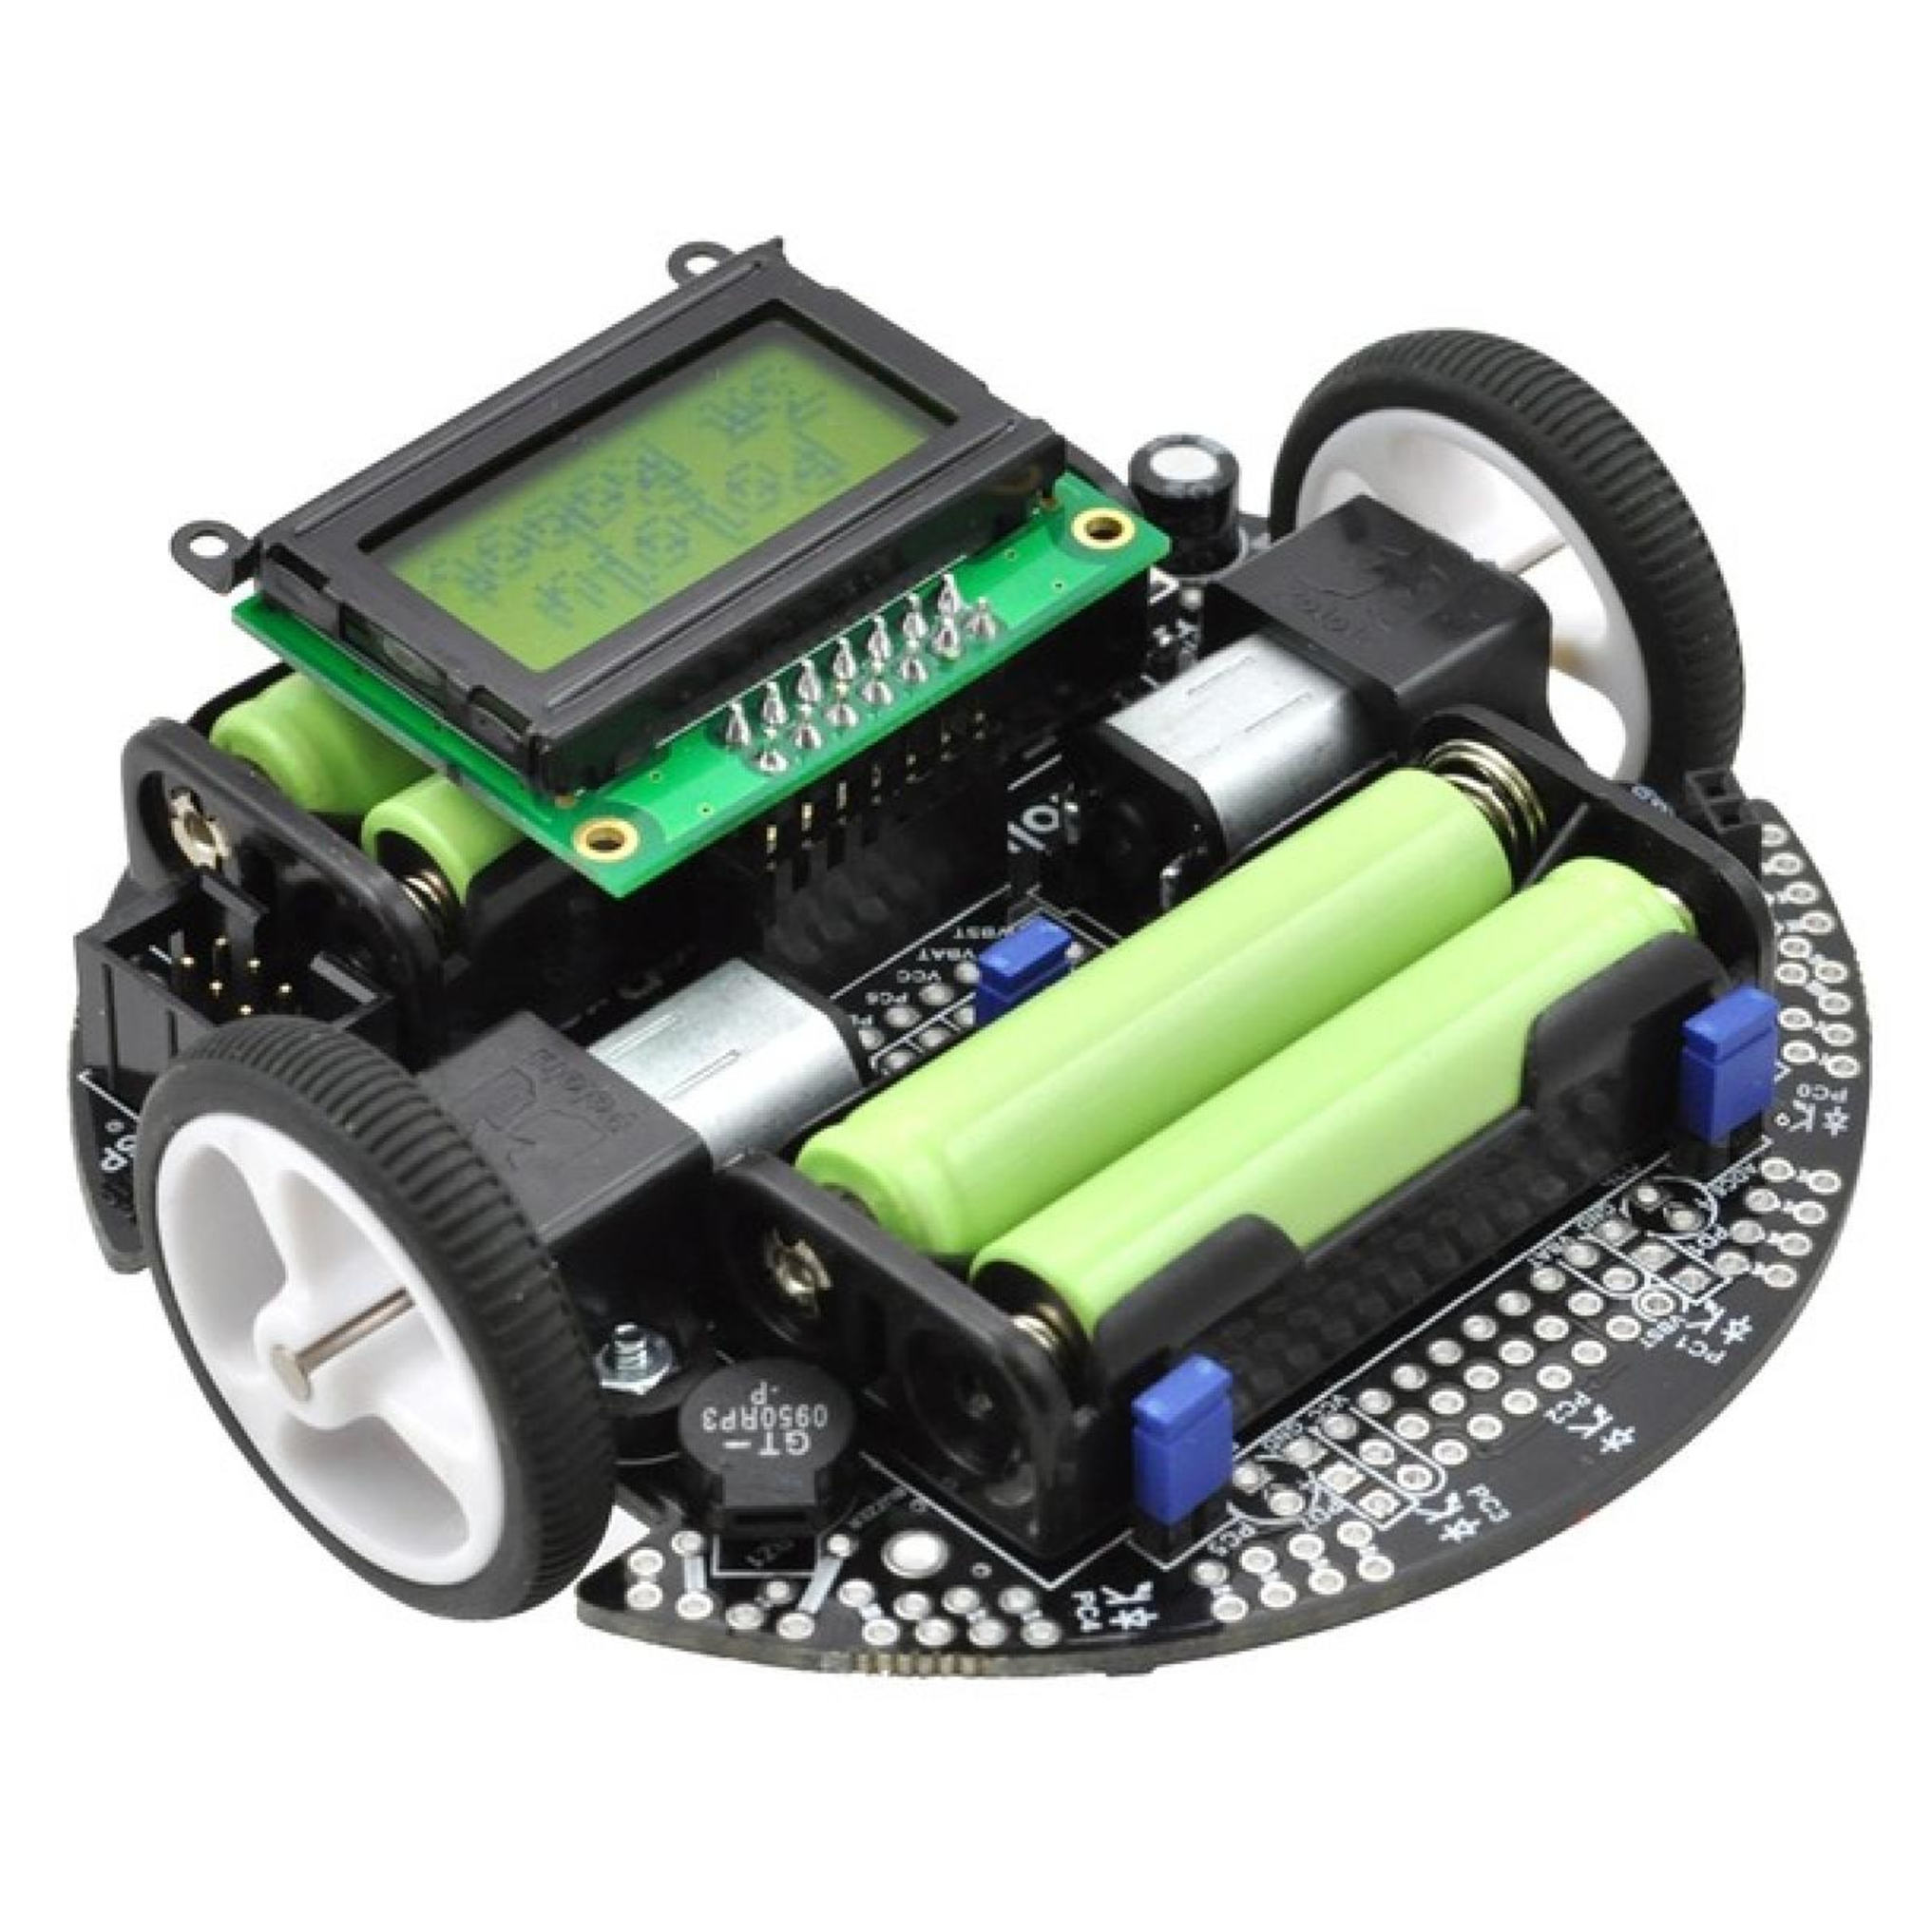
\includegraphics[width=0.35\textwidth]{3pi}
	\end{figure}
\end{frame}

\begin{frame}
	\frametitle{Software}
	\begin{itemize}
		\item  \textbf{Target \& Development-OS}: \textsc{Linux}
		\item  \textbf{IDE}: \textsc{Qt Creator}
		\item  \textbf{Version Control}: \textsc{Git} (hosted on \textit{https://bitbucket.org})
		\item  \textbf{Build System}: \textsc{CMake}
	\end{itemize}
\end{frame}


\section{Tasks} 
\begin{frame}
	\frametitle{Tasks I} 
	Project strategy is based on the spiral model with the following milestones:
	\begin{block}{Deadline: 07.05.2014}
		\begin{itemize}
			\item Kick-off Position
			\item Goalkeeper
			\item Penalty Shooting
		\end{itemize}
	\end{block}
	\begin{block}{Deadline: 04.06.2014}
		\begin{itemize}
			\item Collision Avoidance
			\item Ball Control
			\item Player Interactions
		\end{itemize}
	\end{block}
\end{frame}

\begin{frame}
	\frametitle{Tasks II} 
	\begin{block}{Deadline: 25.06.2014}
		%\begin{itemize}
			Strategy and Tactics
		%\end{itemize}
	\end{block}
	\begin{block}{Deadline: 02.07.2014}
		%\begin{itemize}
			\textsc{RoboSoccer} Championship
		%\end{itemize}
	\end{block}
\end{frame}

\section{Resource Plan} 
\begin{frame}
	\frametitle{Resource Plan I}
	\begin{columns}[t]
		\begin{column}{0.50\textwidth}
			\begin{block}{\textbf{PM} Schmidt Benedikt}
				\begin{itemize}
					\item Communication with the contact person and the tutor of the course.
					\item General team coordination.
					\item Monitor realization of project plan.
				\end{itemize}
			\end{block}
		\end{column}
		
		\begin{column}{0.50\textwidth}
			\begin{block}{\textbf{QM} Wirnshofer Florian}
				\begin{itemize}
					\item Ensure sufficient unit tests.
					\item Continuous testing on hardware.
					\item Balance quality aspiration and effort.
				\end{itemize}
			\end{block}
		\end{column}
	\end{columns}
\end{frame}
\begin{frame}
	\frametitle{Resource Plan II}
	\begin{columns}[t]
		\begin{column}{0.50\textwidth}
			\begin{block}{\textbf{CM} Meyer Kevin}
				\begin{itemize}
					\item Communication with the contact person and the tutor of the course.
					\item General team coordination.
					\item Monitor realization of project plan.
				\end{itemize}
			\end{block}
		\end{column}
		
		\begin{column}{0.50\textwidth}
			\begin{block}{\textbf{SD} Hofbauer Markus, Jiang He}
				\begin{itemize}
					\item Design and verify code structure.
					\item Ensure building code.
					\item Choose and connect external libraries.
				\end{itemize}
			\end{block}
		\end{column}
	\end{columns}
\end{frame}

\section{Time Schedule} 
\begin{frame}
	\frametitle{Time Schedule} 
	\begin{figure}
		\centering
		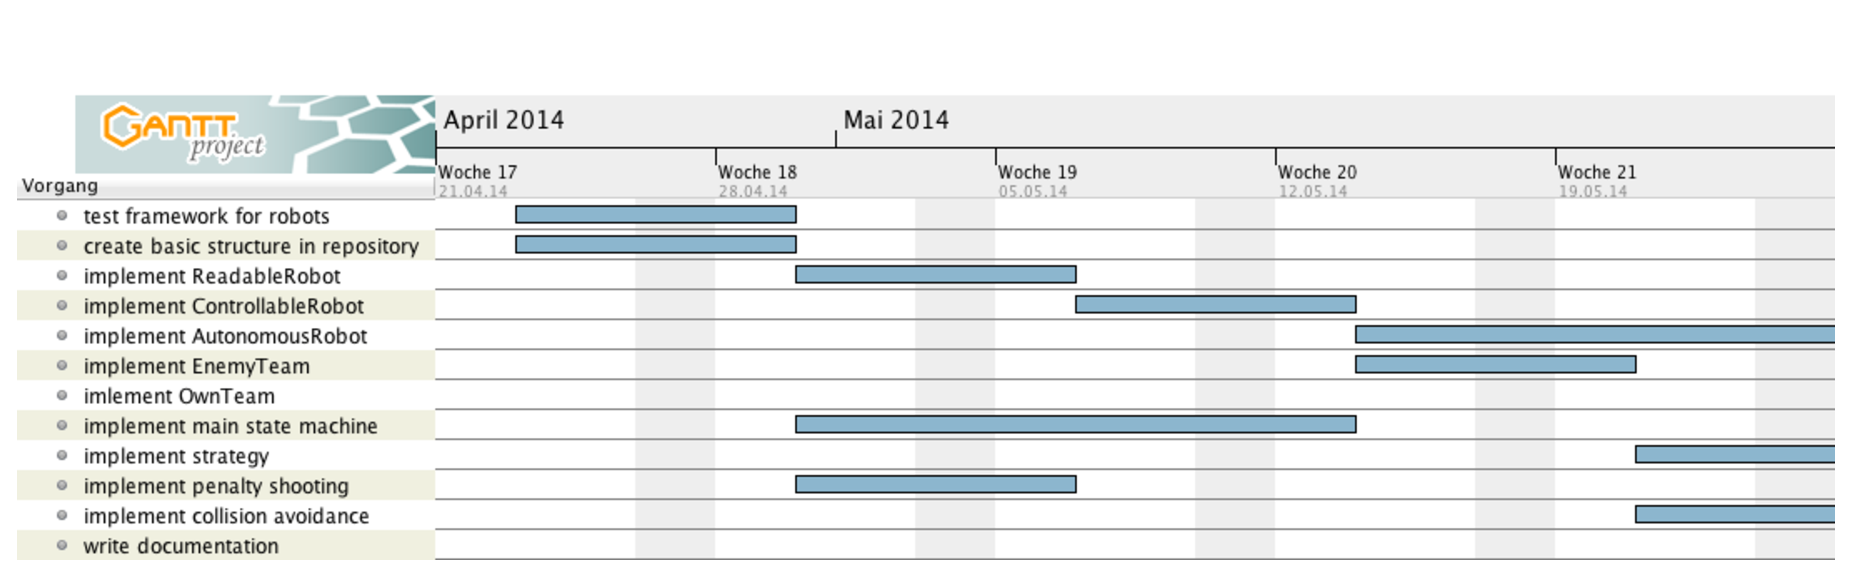
\includegraphics[width = 0.98\textwidth]{g1}
	\end{figure}
	\begin{figure}
		\centering
		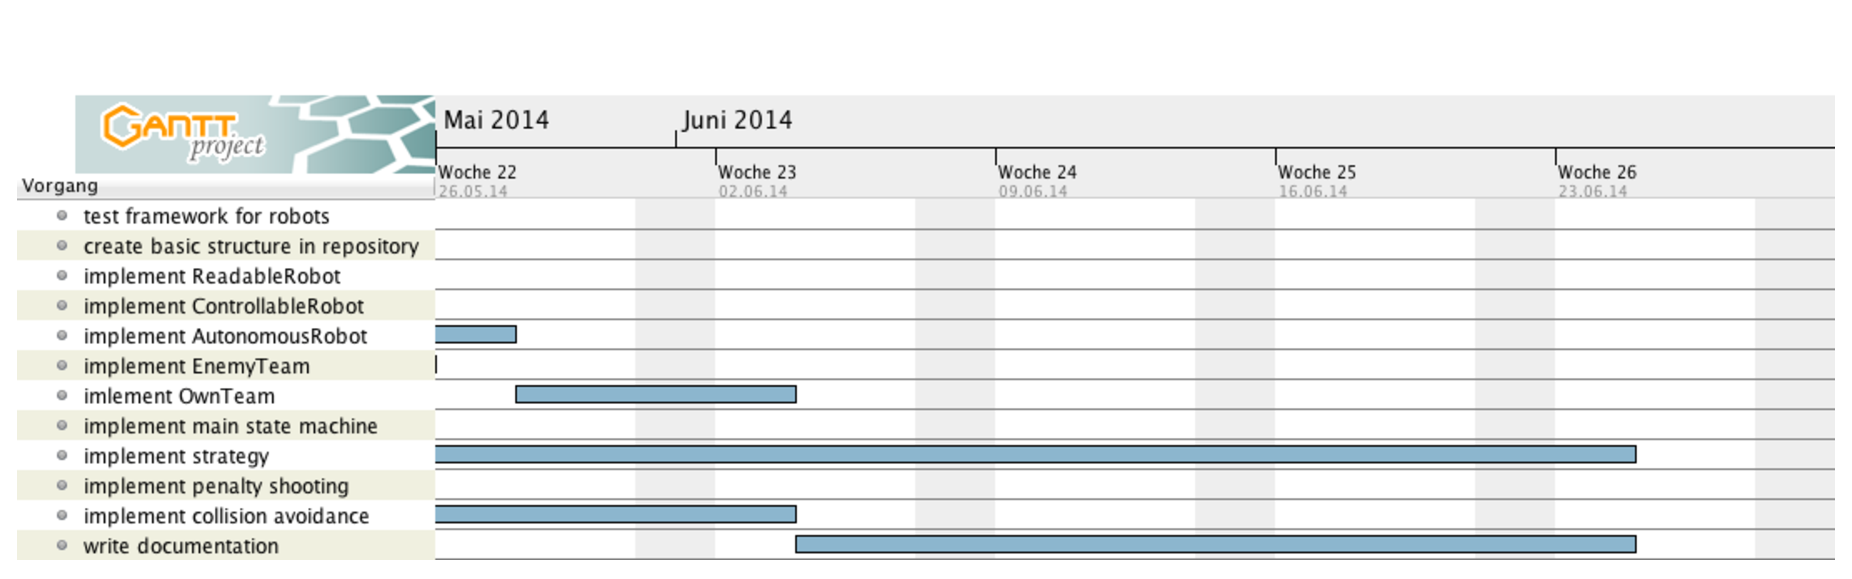
\includegraphics[width = 0.98\textwidth]{g2}
	\end{figure}
	
\end{frame}

\section{Cost Plan} 
\begin{frame}
	\frametitle{Cost Plan} 
	\begin{itemize}
		\item Discussion and creating of implementation issues at each team meeting.
		\item Resolving implementation issues till subsequent team meeting.
	\end{itemize}
	\begin{center}
	\LARGE$\Downarrow$
	\end{center}		
	
	\begin{itemize}
		\item Good knowledge of project status.
		\item Insight in all project tasks.
		\item Scalability of effort required for individual tasks.
	\end{itemize}
\end{frame}

\section{Implementation} 
\begin{frame}
	\frametitle{Implementation}
	\begin{figure}
	\centering
	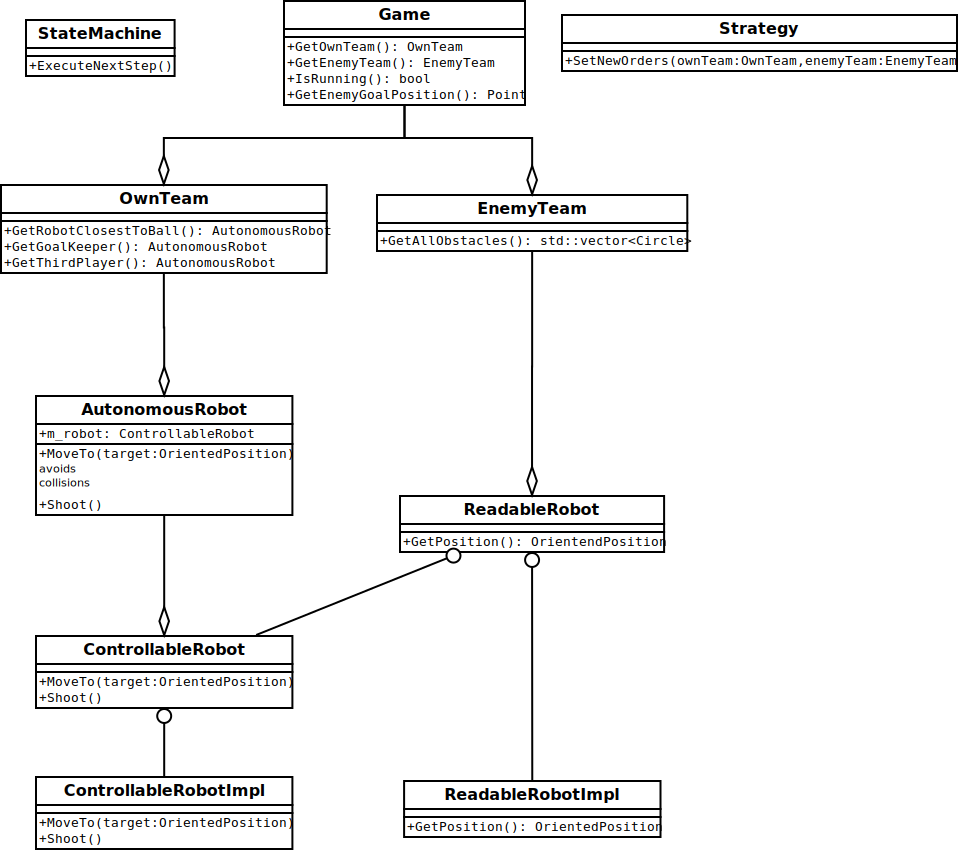
\includegraphics[width = 0.9\textwidth]{architecture}
	\end{figure}
\end{frame}


\end{document}

